\documentclass[11pt,a4paper]{article}
\usepackage[ngerman]{babel}
\usepackage[TS1,T1]{fontenc}
\usepackage[utf8x]{inputenc}
\selectlanguage{ngerman}
\usepackage{theorem}
\usepackage[scaled=0.9]{helvet}
\usepackage{amsmath}
\usepackage{amssymb}
\usepackage{hyperref}
\usepackage{stmaryrd}
\usepackage{pgf,tikz}
\usepackage{relsize}
\usepackage{enumitem}
\usepackage{graphicx}
\usepackage{algpseudocode,amsmath,xifthen}

\newcounter{numb}
\theoremstyle{break}
\theorembodyfont{\upshape}
   	\newtheorem{exercise}{Exercise}[numb]
\setlength{\oddsidemargin}{0cm}
\setlength{\textwidth}{16cm}
\setlength{\textheight}{23cm}
\setlength{\topmargin}{-2cm}

\usetikzlibrary{shapes,arrows,automata,positioning,decorations.fractals}
\renewcommand\familydefault{\sfdefault}

\newcommand{\header}[2]{
\begin{minipage}[b]{\textwidth}
		\parbox[t]{5cm}{%
			
\includegraphics[width=4cm]{unilogo}
			\hfill
		}
		\parbox[b]{11cm}{%
			%\scshape%
			Heinrich-Heine-University D\"usseldorf\\
			Computer Science Department\\
			Software Engineering and Programming Languages\\
			%Professor Dr.\ M.\ Leuschel
		Philipp K\"orner
}
		
\end{minipage}
	\begin{center}
		\bf
		Functional Programming -- WT 2024 / 2025\\
        Reading Guide {\thenumb}: {#1}
	\end{center}

    \pagestyle{empty}
    \paragraph{Timeline:} This unit should be completed by {#2}.
}

\setcounter{numb}{7}


\begin{document}

\begin{minipage}[b]{\textwidth}
	\parbox[t]{5cm}{%
		
\includegraphics[width=4cm]{unilogo}
		\hfill
	}
	\parbox[b]{11cm}{%
		%\scshape%
		Heinrich-Heine-University D\"usseldorf\\
		Computer Science Department\\
		Software Engineering and Programming Languages\\
		%Professor Dr.\ M.\ Leuschel
		Philipp K\"orner
	}
\end{minipage}
\begin{center}
	\bf
	Functional Programming -- WT 2023 / 2024\\
	Reading Guide 7: Macros
\end{center}

\pagestyle{empty}

\paragraph{Timeline:} This unit should be completed by 27.11.2023.

\section{Material} 

\begin{itemize}
    \item 17\_homoiconicity.clj
    \item 11\_macros.clj
    \item Clojure for the Brave and True, chapter 8 (contains next week's material as well)
	\item Clojure Reference: Macros \url{https://clojure.org/reference/macros}
    \item Learning Video: Macros: \url{https://mediathek.hhu.de/watch/7e4ba161-f91b-4c7a-a1e2-e135c861865c}
\end{itemize}


\section{Learning Outcomes}

After completing this unit you should be able to

\begin{itemize}
	\item fully describe the process of evaluation of expressions in Clojure.
    \item define and identify homoiconicity.
    %\item name the values that are generated by the reader.
    %\item read and use reader-macros correctly.
    \item write macros by yourself.
    %\item identify unhygienic macros and rewrite them to be hygienic.
\end{itemize}

\section{Highlights}

\begin{itemize}
    \item Macroexpension
    \item Complete evaluation rules
    \item Helpers: \verb|macroexpand|, \verb|macroexpand-1|, \verb|macroexpand-all|
    \item Macro: \verb|defmacro|
    %\item Reader syntax: \verb|`| (Syntax-Quote), \verb|'| (Quote), \verb|~| (Unquote), \verb|~@| (Unquote-Splicing), \verb|#| (Gensym)
\end{itemize}



\section{Exercises}

\emph{Note:} the next reading guide will contain the same exercises.
You may --- for didactical purposes --- try these exercises now 
to experience the pain of writing macros
without the templating syntax.

\begin{exercise}[Macro]
\begin{enumerate}[label=\alph*)]
\item
Write a macro that implements a simple calculator with infix notation. The first argument should be a vector with bindings of symbols to values. Parentheses and operator precedences need not be considered. The macro should work as follows:
\begin{verbatim}
user=> (calc [a 3] 3 + 5 * a)
24
user=> (calc [b 5 a 3] a * b + 3)
18
\end{verbatim}
\item Why can you not write this calculator as a function?
\end{enumerate}
\end{exercise}

\begin{exercise}[DFA]
Your task is to develop a simple DSL for DFAs.
The automaton that recognizes binary numbers divisible by five will serve as example.
The states in the automaton are labeled according to the residue class modulo 5,
so z0 represents all numbers divisible by 5, z3 all numbers whose remainder is 3, etc.

\begin{minipage}{.4\textwidth}
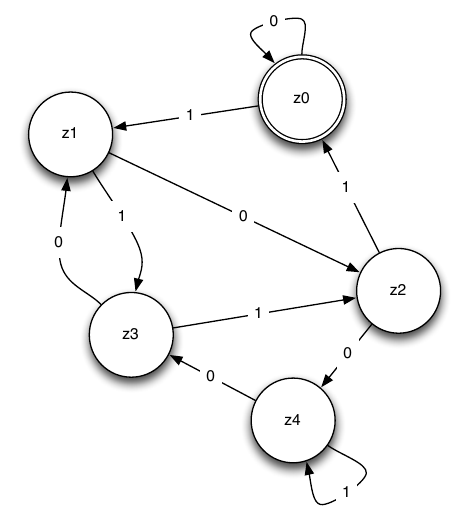
\includegraphics[scale=0.5]{dfa.png} 
\end{minipage}%
\begin{minipage}{.6\textwidth}
    The DSL should look as follows (i.e., \emph{this exact code is expected to work without any modification!} 
    It may only be executed once, so once you have a solution, re-start your REPL to ensure you do not have any left-over state.):

\begin{verbatim}
(declare z0 z1 z2 z3 z4)
(def z0 (dfa-state :accept {\0 z0 \1 z1}))
(def z1 (dfa-state :reject {\0 z2 \1 z3}))
(def z2 (dfa-state :reject {\0 z4 \1 z0}))
(def z3 (dfa-state :reject {\0 z1 \1 z2}))
(def z4 (dfa-state :reject {\0 z3 \1 z4}))
\end{verbatim}

\emph{Nota bene:} You have to use the code snippet above verbatim! No modifications are allowed.

\verb|(dfa-state ... )| should return a function,
which receives a string, consisting of 0s and 1s, as parameter and returns :accept,
if the string starting from this node results in an accepting state.
Otherwise :reject should be returned.
\end{minipage}

\verb|(dfa-match init text)| should serve as entry point, which, starting from init, processes the input text.

\begin{verbatim}
user=> (dfa-match z0 "")
:accept
user=> (dfa-match z0 "010100010")
:reject
user=> (dfa-match z0 "0101000101")
:accept
\end{verbatim}


Test your implementation with larger inputs (i.e. longer strings).

Note: It is likely that your first implementation will not work.
Do not let yourself be discouraged by this and try to locate the problem,
in order to fix it afterwards.

\end{exercise}


	\section*{Questions}
	If you have any questions, please contact Philipp K"orner (\texttt{p.koerner@hhu.de}) or post it to the Rocket.Chat group.
\end{document}

